\documentclass[1p]{elsarticle_modified}
%\bibliographystyle{elsarticle-num}

%\usepackage[colorlinks]{hyperref}
%\usepackage{abbrmath_seonhwa} %\Abb, \Ascr, \Acal ,\Abf, \Afrak
\usepackage{amsfonts}
\usepackage{amssymb}
\usepackage{amsmath}
\usepackage{amsthm}
\usepackage{scalefnt}
\usepackage{amsbsy}
\usepackage{kotex}
\usepackage{caption}
\usepackage{subfig}
\usepackage{color}
\usepackage{graphicx}
\usepackage{xcolor} %% white, black, red, green, blue, cyan, magenta, yellow
\usepackage{float}
\usepackage{setspace}
\usepackage{hyperref}

\usepackage{tikz}
\usetikzlibrary{arrows}

\usepackage{multirow}
\usepackage{array} % fixed length table
\usepackage{hhline}

%%%%%%%%%%%%%%%%%%%%%
\makeatletter
\renewcommand*\env@matrix[1][\arraystretch]{%
	\edef\arraystretch{#1}%
	\hskip -\arraycolsep
	\let\@ifnextchar\new@ifnextchar
	\array{*\c@MaxMatrixCols c}}
\makeatother %https://tex.stackexchange.com/questions/14071/how-can-i-increase-the-line-spacing-in-a-matrix
%%%%%%%%%%%%%%%

\usepackage[normalem]{ulem}

\newcommand{\msout}[1]{\ifmmode\text{\sout{\ensuremath{#1}}}\else\sout{#1}\fi}
%SOURCE: \msout is \stkout macro in https://tex.stackexchange.com/questions/20609/strikeout-in-math-mode

\newcommand{\cancel}[1]{
	\ifmmode
	{\color{red}\msout{#1}}
	\else
	{\color{red}\sout{#1}}
	\fi
}

\newcommand{\add}[1]{
	{\color{blue}\uwave{#1}}
}

\newcommand{\replace}[2]{
	\ifmmode
	{\color{red}\msout{#1}}{\color{blue}\uwave{#2}}
	\else
	{\color{red}\sout{#1}}{\color{blue}\uwave{#2}}
	\fi
}

\newcommand{\Sol}{\mathcal{S}} %segment
\newcommand{\D}{D} %diagram
\newcommand{\A}{\mathcal{A}} %arc


%%%%%%%%%%%%%%%%%%%%%%%%%%%%%5 test

\def\sl{\operatorname{\textup{SL}}(2,\Cbb)}
\def\psl{\operatorname{\textup{PSL}}(2,\Cbb)}
\def\quan{\mkern 1mu \triangleright \mkern 1mu}

\theoremstyle{definition}
\newtheorem{thm}{Theorem}[section]
\newtheorem{prop}[thm]{Proposition}
\newtheorem{lem}[thm]{Lemma}
\newtheorem{ques}[thm]{Question}
\newtheorem{cor}[thm]{Corollary}
\newtheorem{defn}[thm]{Definition}
\newtheorem{exam}[thm]{Example}
\newtheorem{rmk}[thm]{Remark}
\newtheorem{alg}[thm]{Algorithm}

\newcommand{\I}{\sqrt{-1}}
\begin{document}

%\begin{frontmatter}
%
%\title{Boundary parabolic representations of knots up to 8 crossings}
%
%%% Group authors per affiliation:
%\author{Yunhi Cho} 
%\address{Department of Mathematics, University of Seoul, Seoul, Korea}
%\ead{yhcho@uos.ac.kr}
%
%
%\author{Seonhwa Kim} %\fnref{s_kim}}
%\address{Center for Geometry and Physics, Institute for Basic Science, Pohang, 37673, Korea}
%\ead{ryeona17@ibs.re.kr}
%
%\author{Hyuk Kim}
%\address{Department of Mathematical Sciences, Seoul National University, Seoul 08826, Korea}
%\ead{hyukkim@snu.ac.kr}
%
%\author{Seokbeom Yoon}
%\address{Department of Mathematical Sciences, Seoul National University, Seoul, 08826,  Korea}
%\ead{sbyoon15@snu.ac.kr}
%
%\begin{abstract}
%We find all boundary parabolic representation of knots up to 8 crossings.
%
%\end{abstract}
%\begin{keyword}
%    \MSC[2010] 57M25 
%\end{keyword}
%
%\end{frontmatter}

%\linenumbers
%\tableofcontents
%
\newcommand\colored[1]{\textcolor{white}{\rule[-0.35ex]{0.8em}{1.4ex}}\kern-0.8em\color{red} #1}%
%\newcommand\colored[1]{\textcolor{white}{ #1}\kern-2.17ex	\textcolor{white}{ #1}\kern-1.81ex	\textcolor{white}{ #1}\kern-2.15ex\color{red}#1	}

{\Large $\underline{12n_{0436}~(K12n_{0436})}$}

\setlength{\tabcolsep}{10pt}
\renewcommand{\arraystretch}{1.6}
\vspace{1cm}\begin{tabular}{m{100pt}>{\centering\arraybackslash}m{274pt}}
\multirow{5}{120pt}{
	\centering
	\includegraphics[width=112pt]{../../../GIT/diagram.site/Diagrams/png/2525_12n_0436.png}\\
\ \ \ A knot diagram\footnotemark}&
\allowdisplaybreaks
\textbf{Linearized knot diagam} \\
\cline{2-2}
 &
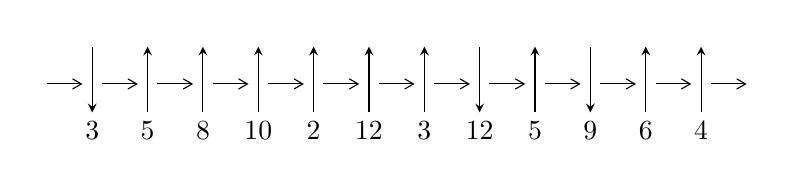
\begin{tikzpicture}[x=20pt, y=17pt]
	% nodes
	\node (C0) at (0, 0) {};
	\node (C1) at (1, 0) {};
	\node (C1U) at (1, +1) {};
	\node (C1D) at (1, -1) {3};

	\node (C2) at (2, 0) {};
	\node (C2U) at (2, +1) {};
	\node (C2D) at (2, -1) {5};

	\node (C3) at (3, 0) {};
	\node (C3U) at (3, +1) {};
	\node (C3D) at (3, -1) {8};

	\node (C4) at (4, 0) {};
	\node (C4U) at (4, +1) {};
	\node (C4D) at (4, -1) {10};

	\node (C5) at (5, 0) {};
	\node (C5U) at (5, +1) {};
	\node (C5D) at (5, -1) {2};

	\node (C6) at (6, 0) {};
	\node (C6U) at (6, +1) {};
	\node (C6D) at (6, -1) {12};

	\node (C7) at (7, 0) {};
	\node (C7U) at (7, +1) {};
	\node (C7D) at (7, -1) {3};

	\node (C8) at (8, 0) {};
	\node (C8U) at (8, +1) {};
	\node (C8D) at (8, -1) {12};

	\node (C9) at (9, 0) {};
	\node (C9U) at (9, +1) {};
	\node (C9D) at (9, -1) {5};

	\node (C10) at (10, 0) {};
	\node (C10U) at (10, +1) {};
	\node (C10D) at (10, -1) {9};

	\node (C11) at (11, 0) {};
	\node (C11U) at (11, +1) {};
	\node (C11D) at (11, -1) {6};

	\node (C12) at (12, 0) {};
	\node (C12U) at (12, +1) {};
	\node (C12D) at (12, -1) {4};
	\node (C13) at (13, 0) {};

	% arrows
	\draw[->,>={angle 60}]
	(C0) edge (C1) (C1) edge (C2) (C2) edge (C3) (C3) edge (C4) (C4) edge (C5) (C5) edge (C6) (C6) edge (C7) (C7) edge (C8) (C8) edge (C9) (C9) edge (C10) (C10) edge (C11) (C11) edge (C12) (C12) edge (C13) ;	\draw[->,>=stealth]
	(C1U) edge (C1D) (C2D) edge (C2U) (C3D) edge (C3U) (C4D) edge (C4U) (C5D) edge (C5U) (C6D) edge (C6U) (C7D) edge (C7U) (C8U) edge (C8D) (C9D) edge (C9U) (C10U) edge (C10D) (C11D) edge (C11U) (C12D) edge (C12U) ;
	\end{tikzpicture} \\
\hhline{~~} \\& 
\textbf{Solving Sequence} \\ \cline{2-2} 
 &
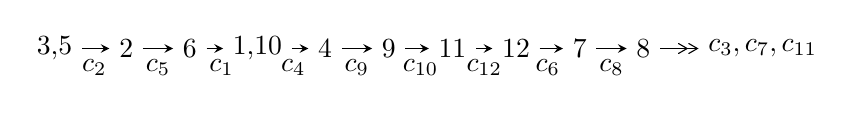
\begin{tikzpicture}[x=23pt, y=7pt]
	% node
	\node (A0) at (-1/8, 0) {3,5};
	\node (A1) at (1, 0) {2};
	\node (A2) at (2, 0) {6};
	\node (A3) at (49/16, 0) {1,10};
	\node (A4) at (33/8, 0) {4};
	\node (A5) at (41/8, 0) {9};
	\node (A6) at (49/8, 0) {11};
	\node (A7) at (57/8, 0) {12};
	\node (A8) at (65/8, 0) {7};
	\node (A9) at (73/8, 0) {8};
	\node (C1) at (1/2, -1) {$c_{2}$};
	\node (C2) at (3/2, -1) {$c_{5}$};
	\node (C3) at (5/2, -1) {$c_{1}$};
	\node (C4) at (29/8, -1) {$c_{4}$};
	\node (C5) at (37/8, -1) {$c_{9}$};
	\node (C6) at (45/8, -1) {$c_{10}$};
	\node (C7) at (53/8, -1) {$c_{12}$};
	\node (C8) at (61/8, -1) {$c_{6}$};
	\node (C9) at (69/8, -1) {$c_{8}$};
	\node (A10) at (11, 0) {$c_{3},c_{7},c_{11}$};

	% edge
	\draw[->,>=stealth]	
	(A0) edge (A1) (A1) edge (A2) (A2) edge (A3) (A3) edge (A4) (A4) edge (A5) (A5) edge (A6) (A6) edge (A7) (A7) edge (A8) (A8) edge (A9) ;
	\draw[->>,>={angle 60}]	
	(A9) edge (A10);
\end{tikzpicture} \\ 

\end{tabular} \\

\footnotetext{
The image of knot diagram is generated by the software ``\textbf{Draw programme}" developed by Andrew Bartholomew(\url{http://www.layer8.co.uk/maths/draw/index.htm\#Running-draw}), where we modified some parts for our purpose(\url{https://github.com/CATsTAILs/LinksPainter}).
}\phantom \\ \newline 
\centering \textbf{Ideals for irreducible components\footnotemark of $X_{\text{par}}$} 
 
\begin{align*}
I^u_{1}&=\langle 
-37827406 u^{18}+29757877 u^{17}+\cdots+120133473 b+294183386,\;a-1,\;u^{19}+6 u^{17}+\cdots+2 u+1\rangle \\
I^u_{2}&=\langle 
- u^4- u^3-2 u^2+b-2 u+2,\;a+1,\;u^5+u^4+2 u^3+3 u^2+u+1\rangle \\
I^u_{3}&=\langle 
b-1,\;19 u^{11}-5 u^{10}+80 u^9-30 u^8+158 u^7-42 u^6+229 u^5-4 u^4+188 u^3+17 u^2+5 a+39 u+21,\\
\phantom{I^u_{3}}&\phantom{= \langle  }u^{12}- u^{11}+5 u^{10}-5 u^9+12 u^8-10 u^7+19 u^6-12 u^5+18 u^4-9 u^3+8 u^2-2 u+1\rangle \\
I^u_{4}&=\langle 
b+1,\;858366437 u^{13}+13303924407 u^{12}+\cdots+198592491933 a-215876970671,\\
\phantom{I^u_{4}}&\phantom{= \langle  }u^{14}-5 u^{12}+u^{11}+20 u^{10}-3 u^9-41 u^8+3 u^7+27 u^6+15 u^5+23 u^4-53 u^3-33 u^2+71 u-27\rangle \\
I^u_{5}&=\langle 
b-1,\;a+u,\;u^2+u+1\rangle \\
\\
\end{align*}
\raggedright * 5 irreducible components of $\dim_{\mathbb{C}}=0$, with total 52 representations.\\
\footnotetext{All coefficients of polynomials are rational numbers. But the coefficients are sometimes approximated in decimal forms when there is not enough margin.}
\newpage
\renewcommand{\arraystretch}{1}
\centering \section*{I. $I^u_{1}= \langle -3.78\times10^{7} u^{18}+2.98\times10^{7} u^{17}+\cdots+1.20\times10^{8} b+2.94\times10^{8},\;a-1,\;u^{19}+6 u^{17}+\cdots+2 u+1 \rangle$}
\flushleft \textbf{(i) Arc colorings}\\
\begin{tabular}{m{7pt} m{180pt} m{7pt} m{180pt} }
\flushright $a_{3}=$&$\begin{pmatrix}1\\0\end{pmatrix}$ \\
\flushright $a_{5}=$&$\begin{pmatrix}0\\u\end{pmatrix}$ \\
\flushright $a_{2}=$&$\begin{pmatrix}1\\u^2\end{pmatrix}$ \\
\flushright $a_{6}=$&$\begin{pmatrix}u\\u^3+u\end{pmatrix}$ \\
\flushright $a_{1}=$&$\begin{pmatrix}u^2+1\\u^2\end{pmatrix}$ \\
\flushright $a_{10}=$&$\begin{pmatrix}1\\0.314878 u^{18}-0.247707 u^{17}+\cdots-3.86583 u-2.44880\end{pmatrix}$ \\
\flushright $a_{4}=$&$\begin{pmatrix}- u\\0.247707 u^{18}-0.105766 u^{17}+\cdots+4.07856 u+0.314878\end{pmatrix}$ \\
\flushright $a_{9}=$&$\begin{pmatrix}1\\0.314878 u^{18}-0.247707 u^{17}+\cdots-3.86583 u-2.44880\end{pmatrix}$ \\
\flushright $a_{11}=$&$\begin{pmatrix}u^2+1\\0.420645 u^{18}-0.371361 u^{17}+\cdots-3.68529 u-2.20110\end{pmatrix}$ \\
\flushright $a_{12}=$&$\begin{pmatrix}-0.00612192 u^{18}+0.0147829 u^{17}+\cdots+0.322078 u+1.37136\\0.297103 u^{18}-0.361177 u^{17}+\cdots-3.38666 u-1.84452\end{pmatrix}$ \\
\flushright $a_{7}=$&$\begin{pmatrix}0.648921 u^{18}+0.257817 u^{17}+\cdots+6.78287 u+0.742285\\-0.744255 u^{18}+0.115009 u^{17}+\cdots-1.84764 u+0.485311\end{pmatrix}$ \\
\flushright $a_{8}=$&$\begin{pmatrix}0.0953339 u^{18}-0.372826 u^{17}+\cdots-4.93523 u-1.22760\\0.744255 u^{18}-0.115009 u^{17}+\cdots+1.84764 u-0.485311\end{pmatrix}$\\&\end{tabular}
\flushleft \textbf{(ii) Obstruction class $= -1$}\\~\\
\flushleft \textbf{(iii) Cusp Shapes $= \frac{42941320}{40044491} u^{18}+\frac{84579765}{40044491} u^{17}+\cdots+\frac{1067191176}{40044491} u+\frac{715529589}{40044491}$}\\~\\
\newpage\renewcommand{\arraystretch}{1}
\flushleft \textbf{(iv) u-Polynomials at the component}\newline \\
\begin{tabular}{m{50pt}|m{274pt}}
Crossings & \hspace{64pt}u-Polynomials at each crossing \\
\hline $$\begin{aligned}c_{1},c_{10}\end{aligned}$$&$\begin{aligned}
&u^{19}+12 u^{18}+\cdots-12 u-1
\end{aligned}$\\
\hline $$\begin{aligned}c_{2},c_{4},c_{5}\\c_{9}\end{aligned}$$&$\begin{aligned}
&u^{19}+6 u^{17}+\cdots+2 u-1
\end{aligned}$\\
\hline $$\begin{aligned}c_{3},c_{7}\end{aligned}$$&$\begin{aligned}
&u^{19}+5 u^{18}+\cdots-5 u-3
\end{aligned}$\\
\hline $$\begin{aligned}c_{6},c_{11},c_{12}\end{aligned}$$&$\begin{aligned}
&u^{19}+u^{18}+\cdots+u-3
\end{aligned}$\\
\hline $$\begin{aligned}c_{8}\end{aligned}$$&$\begin{aligned}
&u^{19}- u^{18}+\cdots-2 u-1
\end{aligned}$\\
\hline
\end{tabular}\\~\\
\newpage\renewcommand{\arraystretch}{1}
\flushleft \textbf{(v) Riley Polynomials at the component}\newline \\
\begin{tabular}{m{50pt}|m{274pt}}
Crossings & \hspace{64pt}Riley Polynomials at each crossing \\
\hline $$\begin{aligned}c_{1},c_{10}\end{aligned}$$&$\begin{aligned}
&y^{19}+32 y^{18}+\cdots+116 y-1
\end{aligned}$\\
\hline $$\begin{aligned}c_{2},c_{4},c_{5}\\c_{9}\end{aligned}$$&$\begin{aligned}
&y^{19}+12 y^{18}+\cdots-12 y-1
\end{aligned}$\\
\hline $$\begin{aligned}c_{3},c_{7}\end{aligned}$$&$\begin{aligned}
&y^{19}-3 y^{18}+\cdots+103 y-9
\end{aligned}$\\
\hline $$\begin{aligned}c_{6},c_{11},c_{12}\end{aligned}$$&$\begin{aligned}
&y^{19}-17 y^{18}+\cdots+73 y-9
\end{aligned}$\\
\hline $$\begin{aligned}c_{8}\end{aligned}$$&$\begin{aligned}
&y^{19}+11 y^{18}+\cdots+44 y-1
\end{aligned}$\\
\hline
\end{tabular}\\~\\
\newpage\flushleft \textbf{(vi) Complex Volumes and Cusp Shapes}
$$\begin{array}{c|c|c}  
\text{Solutions to }I^u_{1}& \I (\text{vol} + \sqrt{-1}CS) & \text{Cusp shape}\\
 \hline 
\begin{aligned}
u &= \phantom{-}0.581330 + 0.811360 I \\
a &= \phantom{-}1.00000\phantom{ +0.000000I} \\
b &= \phantom{-}1.79148 + 0.06667 I\end{aligned}
 & \phantom{-}1.93762 + 6.06371 I & \phantom{-}8.03507 - 11.60220 I \\ \hline\begin{aligned}
u &= \phantom{-}0.581330 - 0.811360 I \\
a &= \phantom{-}1.00000\phantom{ +0.000000I} \\
b &= \phantom{-}1.79148 - 0.06667 I\end{aligned}
 & \phantom{-}1.93762 - 6.06371 I & \phantom{-}8.03507 + 11.60220 I \\ \hline\begin{aligned}
u &= -0.052078 + 1.011790 I \\
a &= \phantom{-}1.00000\phantom{ +0.000000I} \\
b &= -0.842437 + 0.221761 I\end{aligned}
 & -5.84256 - 3.61662 I & -2.20671 + 4.58081 I \\ \hline\begin{aligned}
u &= -0.052078 - 1.011790 I \\
a &= \phantom{-}1.00000\phantom{ +0.000000I} \\
b &= -0.842437 - 0.221761 I\end{aligned}
 & -5.84256 + 3.61662 I & -2.20671 - 4.58081 I \\ \hline\begin{aligned}
u &= -0.565597 + 0.850482 I \\
a &= \phantom{-}1.00000\phantom{ +0.000000I} \\
b &= \phantom{-}1.102220 - 0.467413 I\end{aligned}
 & \phantom{-}1.71886 - 3.11685 I & \phantom{-}6.74582 + 2.04810 I \\ \hline\begin{aligned}
u &= -0.565597 - 0.850482 I \\
a &= \phantom{-}1.00000\phantom{ +0.000000I} \\
b &= \phantom{-}1.102220 + 0.467413 I\end{aligned}
 & \phantom{-}1.71886 + 3.11685 I & \phantom{-}6.74582 - 2.04810 I \\ \hline\begin{aligned}
u &= -0.435881 + 0.933169 I \\
a &= \phantom{-}1.00000\phantom{ +0.000000I} \\
b &= \phantom{-}0.557982 + 0.070489 I\end{aligned}
 & \phantom{-}1.42719 - 4.85166 I & \phantom{-}4.33736 + 8.70146 I \\ \hline\begin{aligned}
u &= -0.435881 - 0.933169 I \\
a &= \phantom{-}1.00000\phantom{ +0.000000I} \\
b &= \phantom{-}0.557982 - 0.070489 I\end{aligned}
 & \phantom{-}1.42719 + 4.85166 I & \phantom{-}4.33736 - 8.70146 I \\ \hline\begin{aligned}
u &= \phantom{-}0.372674 + 0.734435 I \\
a &= \phantom{-}1.00000\phantom{ +0.000000I} \\
b &= \phantom{-}0.950589 - 1.042440 I\end{aligned}
 & \phantom{-}2.83649 + 2.15459 I & \phantom{-}8.45889 - 1.98320 I \\ \hline\begin{aligned}
u &= \phantom{-}0.372674 - 0.734435 I \\
a &= \phantom{-}1.00000\phantom{ +0.000000I} \\
b &= \phantom{-}0.950589 + 1.042440 I\end{aligned}
 & \phantom{-}2.83649 - 2.15459 I & \phantom{-}8.45889 + 1.98320 I\\
 \hline 
 \end{array}$$\newpage$$\begin{array}{c|c|c}  
\text{Solutions to }I^u_{1}& \I (\text{vol} + \sqrt{-1}CS) & \text{Cusp shape}\\
 \hline 
\begin{aligned}
u &= \phantom{-}0.23610 + 1.41105 I \\
a &= \phantom{-}1.00000\phantom{ +0.000000I} \\
b &= \phantom{-}3.07117 + 0.59581 I\end{aligned}
 & -8.40212 + 4.72676 I & \phantom{-}11.67641 + 3.78763 I \\ \hline\begin{aligned}
u &= \phantom{-}0.23610 - 1.41105 I \\
a &= \phantom{-}1.00000\phantom{ +0.000000I} \\
b &= \phantom{-}3.07117 - 0.59581 I\end{aligned}
 & -8.40212 - 4.72676 I & \phantom{-}11.67641 - 3.78763 I \\ \hline\begin{aligned}
u &= \phantom{-}0.010555 + 0.413321 I \\
a &= \phantom{-}1.00000\phantom{ +0.000000I} \\
b &= -1.95315 - 0.78032 I\end{aligned}
 & -2.02437 - 2.68122 I & \phantom{-}11.08292 + 6.93097 I \\ \hline\begin{aligned}
u &= \phantom{-}0.010555 - 0.413321 I \\
a &= \phantom{-}1.00000\phantom{ +0.000000I} \\
b &= -1.95315 + 0.78032 I\end{aligned}
 & -2.02437 + 2.68122 I & \phantom{-}11.08292 - 6.93097 I \\ \hline\begin{aligned}
u &= -0.374990\phantom{ +0.000000I} \\
a &= \phantom{-}1.00000\phantom{ +0.000000I} \\
b &= \phantom{-}0.313865\phantom{ +0.000000I}\end{aligned}
 & \phantom{-}0.679468\phantom{ +0.000000I} & \phantom{-}14.8670\phantom{ +0.000000I} \\ \hline\begin{aligned}
u &= \phantom{-}1.15639 + 1.32365 I \\
a &= \phantom{-}1.00000\phantom{ +0.000000I} \\
b &= \phantom{-}2.04850 + 0.73446 I\end{aligned}
 & \phantom{-}12.4777 + 13.4078 I & \phantom{-}7.73596 - 5.99135 I \\ \hline\begin{aligned}
u &= \phantom{-}1.15639 - 1.32365 I \\
a &= \phantom{-}1.00000\phantom{ +0.000000I} \\
b &= \phantom{-}2.04850 - 0.73446 I\end{aligned}
 & \phantom{-}12.4777 - 13.4078 I & \phantom{-}7.73596 + 5.99135 I \\ \hline\begin{aligned}
u &= -1.11599 + 1.40313 I \\
a &= \phantom{-}1.00000\phantom{ +0.000000I} \\
b &= \phantom{-}2.11672 - 0.67442 I\end{aligned}
 & \phantom{-}11.98080 - 5.53483 I & \phantom{-}7.70079 + 2.32699 I \\ \hline\begin{aligned}
u &= -1.11599 - 1.40313 I \\
a &= \phantom{-}1.00000\phantom{ +0.000000I} \\
b &= \phantom{-}2.11672 + 0.67442 I\end{aligned}
 & \phantom{-}11.98080 + 5.53483 I & \phantom{-}7.70079 - 2.32699 I\\
 \hline 
 \end{array}$$\newpage\newpage\renewcommand{\arraystretch}{1}
\centering \section*{II. $I^u_{2}= \langle - u^4- u^3-2 u^2+b-2 u+2,\;a+1,\;u^5+u^4+2 u^3+3 u^2+u+1 \rangle$}
\flushleft \textbf{(i) Arc colorings}\\
\begin{tabular}{m{7pt} m{180pt} m{7pt} m{180pt} }
\flushright $a_{3}=$&$\begin{pmatrix}1\\0\end{pmatrix}$ \\
\flushright $a_{5}=$&$\begin{pmatrix}0\\u\end{pmatrix}$ \\
\flushright $a_{2}=$&$\begin{pmatrix}1\\u^2\end{pmatrix}$ \\
\flushright $a_{6}=$&$\begin{pmatrix}u\\u^3+u\end{pmatrix}$ \\
\flushright $a_{1}=$&$\begin{pmatrix}u^2+1\\u^2\end{pmatrix}$ \\
\flushright $a_{10}=$&$\begin{pmatrix}-1\\u^4+u^3+2 u^2+2 u-2\end{pmatrix}$ \\
\flushright $a_{4}=$&$\begin{pmatrix}- u\\- u^2-2 u-1\end{pmatrix}$ \\
\flushright $a_{9}=$&$\begin{pmatrix}-1\\u^4+u^3+u^2+2 u-2\end{pmatrix}$ \\
\flushright $a_{11}=$&$\begin{pmatrix}- u^2-1\\- u^2+u-2\end{pmatrix}$ \\
\flushright $a_{12}=$&$\begin{pmatrix}0\\u^4+u^2+u-1\end{pmatrix}$ \\
\flushright $a_{7}=$&$\begin{pmatrix}u\\- u-1\end{pmatrix}$ \\
\flushright $a_{8}=$&$\begin{pmatrix}-1\\- u-1\end{pmatrix}$\\&\end{tabular}
\flushleft \textbf{(ii) Obstruction class $= 1$}\\~\\
\flushleft \textbf{(iii) Cusp Shapes $= 5 u^4+6 u^3+10 u^2+5 u-2$}\\~\\
\newpage\renewcommand{\arraystretch}{1}
\flushleft \textbf{(iv) u-Polynomials at the component}\newline \\
\begin{tabular}{m{50pt}|m{274pt}}
Crossings & \hspace{64pt}u-Polynomials at each crossing \\
\hline $$\begin{aligned}c_{1}\end{aligned}$$&$\begin{aligned}
&u^5-3 u^4+7 u^2-5 u+1
\end{aligned}$\\
\hline $$\begin{aligned}c_{2},c_{4}\end{aligned}$$&$\begin{aligned}
&u^5+u^4+2 u^3+3 u^2+u+1
\end{aligned}$\\
\hline $$\begin{aligned}c_{3}\end{aligned}$$&$\begin{aligned}
&u^5+4 u^4+8 u^3+7 u^2+2 u-1
\end{aligned}$\\
\hline $$\begin{aligned}c_{5},c_{9}\end{aligned}$$&$\begin{aligned}
&u^5- u^4+2 u^3-3 u^2+u-1
\end{aligned}$\\
\hline $$\begin{aligned}c_{6},c_{12}\end{aligned}$$&$\begin{aligned}
&u^5+2 u^4+u^3+2 u^2+1
\end{aligned}$\\
\hline $$\begin{aligned}c_{7}\end{aligned}$$&$\begin{aligned}
&u^5-4 u^4+8 u^3-7 u^2+2 u+1
\end{aligned}$\\
\hline $$\begin{aligned}c_{8}\end{aligned}$$&$\begin{aligned}
&u^5-3 u^3+u^2+3 u+1
\end{aligned}$\\
\hline $$\begin{aligned}c_{10}\end{aligned}$$&$\begin{aligned}
&u^5+3 u^4-7 u^2-5 u-1
\end{aligned}$\\
\hline $$\begin{aligned}c_{11}\end{aligned}$$&$\begin{aligned}
&u^5-2 u^4+u^3-2 u^2-1
\end{aligned}$\\
\hline
\end{tabular}\\~\\
\newpage\renewcommand{\arraystretch}{1}
\flushleft \textbf{(v) Riley Polynomials at the component}\newline \\
\begin{tabular}{m{50pt}|m{274pt}}
Crossings & \hspace{64pt}Riley Polynomials at each crossing \\
\hline $$\begin{aligned}c_{1},c_{10}\end{aligned}$$&$\begin{aligned}
&y^5-9 y^4+32 y^3-43 y^2+11 y-1
\end{aligned}$\\
\hline $$\begin{aligned}c_{2},c_{4},c_{5}\\c_{9}\end{aligned}$$&$\begin{aligned}
&y^5+3 y^4-7 y^2-5 y-1
\end{aligned}$\\
\hline $$\begin{aligned}c_{3},c_{7}\end{aligned}$$&$\begin{aligned}
&y^5+12 y^3-9 y^2+18 y-1
\end{aligned}$\\
\hline $$\begin{aligned}c_{6},c_{11},c_{12}\end{aligned}$$&$\begin{aligned}
&y^5-2 y^4-7 y^3-8 y^2-4 y-1
\end{aligned}$\\
\hline $$\begin{aligned}c_{8}\end{aligned}$$&$\begin{aligned}
&y^5-6 y^4+15 y^3-19 y^2+7 y-1
\end{aligned}$\\
\hline
\end{tabular}\\~\\
\newpage\flushleft \textbf{(vi) Complex Volumes and Cusp Shapes}
$$\begin{array}{c|c|c}  
\text{Solutions to }I^u_{2}& \I (\text{vol} + \sqrt{-1}CS) & \text{Cusp shape}\\
 \hline 
\begin{aligned}
u &= -1.23887\phantom{ +0.000000I} \\
a &= -1.00000\phantom{ +0.000000I} \\
b &= -0.953942\phantom{ +0.000000I}\end{aligned}
 & \phantom{-}5.64999\phantom{ +0.000000I} & \phantom{-}7.52320\phantom{ +0.000000I} \\ \hline\begin{aligned}
u &= -0.082938 + 0.638199 I \\
a &= -1.00000\phantom{ +0.000000I} \\
b &= -2.71682 + 0.90269 I\end{aligned}
 & -2.41512 + 2.46056 I & -5.06862 + 1.07566 I \\ \hline\begin{aligned}
u &= -0.082938 - 0.638199 I \\
a &= -1.00000\phantom{ +0.000000I} \\
b &= -2.71682 - 0.90269 I\end{aligned}
 & -2.41512 - 2.46056 I & -5.06862 - 1.07566 I \\ \hline\begin{aligned}
u &= \phantom{-}0.202374 + 1.381280 I \\
a &= -1.00000\phantom{ +0.000000I} \\
b &= -3.30621 - 0.67253 I\end{aligned}
 & -8.63454 + 4.90423 I & -10.6930 - 12.7347 I \\ \hline\begin{aligned}
u &= \phantom{-}0.202374 - 1.381280 I \\
a &= -1.00000\phantom{ +0.000000I} \\
b &= -3.30621 + 0.67253 I\end{aligned}
 & -8.63454 - 4.90423 I & -10.6930 + 12.7347 I\\
 \hline 
 \end{array}$$\newpage\newpage\renewcommand{\arraystretch}{1}
\centering \section*{III. $I^u_{3}= \langle b-1,\;19 u^{11}-5 u^{10}+\cdots+5 a+21,\;u^{12}- u^{11}+\cdots-2 u+1 \rangle$}
\flushleft \textbf{(i) Arc colorings}\\
\begin{tabular}{m{7pt} m{180pt} m{7pt} m{180pt} }
\flushright $a_{3}=$&$\begin{pmatrix}1\\0\end{pmatrix}$ \\
\flushright $a_{5}=$&$\begin{pmatrix}0\\u\end{pmatrix}$ \\
\flushright $a_{2}=$&$\begin{pmatrix}1\\u^2\end{pmatrix}$ \\
\flushright $a_{6}=$&$\begin{pmatrix}u\\u^3+u\end{pmatrix}$ \\
\flushright $a_{1}=$&$\begin{pmatrix}u^2+1\\u^2\end{pmatrix}$ \\
\flushright $a_{10}=$&$\begin{pmatrix}-\frac{19}{5} u^{11}+u^{10}+\cdots-\frac{39}{5} u-\frac{21}{5}\\1\end{pmatrix}$ \\
\flushright $a_{4}=$&$\begin{pmatrix}\frac{2}{5} u^{11}+2 u^{10}+\cdots-\frac{53}{5} u+\frac{33}{5}\\\frac{14}{5} u^{11}-3 u^{10}+\cdots+\frac{64}{5} u-\frac{19}{5}\end{pmatrix}$ \\
\flushright $a_{9}=$&$\begin{pmatrix}-\frac{19}{5} u^{11}+u^{10}+\cdots-\frac{39}{5} u-\frac{21}{5}\\\frac{1}{5} u^{11}+u^{10}+\cdots-\frac{9}{5} u+\frac{19}{5}\end{pmatrix}$ \\
\flushright $a_{11}=$&$\begin{pmatrix}-\frac{3}{5} u^{11}-2 u^9+\cdots+\frac{7}{5} u+\frac{8}{5}\\-\frac{11}{5} u^{11}+2 u^{10}+\cdots-\frac{31}{5} u-\frac{4}{5}\end{pmatrix}$ \\
\flushright $a_{12}=$&$\begin{pmatrix}-\frac{3}{5} u^{11}-2 u^9+\cdots+\frac{7}{5} u+\frac{13}{5}\\-\frac{11}{5} u^{11}+2 u^{10}+\cdots-\frac{31}{5} u+\frac{1}{5}\end{pmatrix}$ \\
\flushright $a_{7}=$&$\begin{pmatrix}\frac{16}{5} u^{11}-3 u^{10}+\cdots+\frac{81}{5} u-\frac{36}{5}\\\frac{2}{5} u^{11}+u^{10}+\cdots-\frac{18}{5} u+\frac{18}{5}\end{pmatrix}$ \\
\flushright $a_{8}=$&$\begin{pmatrix}\frac{18}{5} u^{11}-2 u^{10}+\cdots+\frac{63}{5} u-\frac{18}{5}\\\frac{2}{5} u^{11}+u^{10}+\cdots-\frac{18}{5} u+\frac{18}{5}\end{pmatrix}$\\&\end{tabular}
\flushleft \textbf{(ii) Obstruction class $= 1$}\\~\\
\flushleft \textbf{(iii) Cusp Shapes $= \frac{28}{5} u^{11}-10 u^{10}+27 u^9-46 u^8+\frac{331}{5} u^7-\frac{439}{5} u^6+\frac{513}{5} u^5-\frac{573}{5} u^4+\frac{416}{5} u^3-\frac{466}{5} u^2+\frac{153}{5} u-\frac{43}{5}$}\\~\\
\newpage\renewcommand{\arraystretch}{1}
\flushleft \textbf{(iv) u-Polynomials at the component}\newline \\
\begin{tabular}{m{50pt}|m{274pt}}
Crossings & \hspace{64pt}u-Polynomials at each crossing \\
\hline $$\begin{aligned}c_{1}\end{aligned}$$&$\begin{aligned}
&u^{12}-9 u^{11}+\cdots-12 u+1
\end{aligned}$\\
\hline $$\begin{aligned}c_{2},c_{4}\end{aligned}$$&$\begin{aligned}
&u^{12}- u^{11}+\cdots-2 u+1
\end{aligned}$\\
\hline $$\begin{aligned}c_{3}\end{aligned}$$&$\begin{aligned}
&(u^6- u^5+u^4+u^3+u+1)^2
\end{aligned}$\\
\hline $$\begin{aligned}c_{5},c_{9}\end{aligned}$$&$\begin{aligned}
&u^{12}+u^{11}+\cdots+2 u+1
\end{aligned}$\\
\hline $$\begin{aligned}c_{6},c_{12}\end{aligned}$$&$\begin{aligned}
&u^{12}-3 u^{11}+3 u^{10}+u^9-7 u^8+7 u^7+2 u^6-7 u^5+6 u^4-4 u^3+4 u^2+1
\end{aligned}$\\
\hline $$\begin{aligned}c_{7}\end{aligned}$$&$\begin{aligned}
&(u^6+u^5+u^4- u^3- u+1)^2
\end{aligned}$\\
\hline $$\begin{aligned}c_{8}\end{aligned}$$&$\begin{aligned}
&u^{12}-4 u^{11}+\cdots-4 u+1
\end{aligned}$\\
\hline $$\begin{aligned}c_{10}\end{aligned}$$&$\begin{aligned}
&u^{12}+9 u^{11}+\cdots+12 u+1
\end{aligned}$\\
\hline $$\begin{aligned}c_{11}\end{aligned}$$&$\begin{aligned}
&u^{12}+3 u^{11}+3 u^{10}- u^9-7 u^8-7 u^7+2 u^6+7 u^5+6 u^4+4 u^3+4 u^2+1
\end{aligned}$\\
\hline
\end{tabular}\\~\\
\newpage\renewcommand{\arraystretch}{1}
\flushleft \textbf{(v) Riley Polynomials at the component}\newline \\
\begin{tabular}{m{50pt}|m{274pt}}
Crossings & \hspace{64pt}Riley Polynomials at each crossing \\
\hline $$\begin{aligned}c_{1},c_{10}\end{aligned}$$&$\begin{aligned}
&y^{12}-3 y^{11}+\cdots-16 y+1
\end{aligned}$\\
\hline $$\begin{aligned}c_{2},c_{4},c_{5}\\c_{9}\end{aligned}$$&$\begin{aligned}
&y^{12}+9 y^{11}+\cdots+12 y+1
\end{aligned}$\\
\hline $$\begin{aligned}c_{3},c_{7}\end{aligned}$$&$\begin{aligned}
&(y^6+y^5+3 y^4+3 y^3- y+1)^2
\end{aligned}$\\
\hline $$\begin{aligned}c_{6},c_{11},c_{12}\end{aligned}$$&$\begin{aligned}
&y^{12}-3 y^{11}+\cdots+8 y+1
\end{aligned}$\\
\hline $$\begin{aligned}c_{8}\end{aligned}$$&$\begin{aligned}
&y^{12}+2 y^{11}+\cdots+2 y+1
\end{aligned}$\\
\hline
\end{tabular}\\~\\
\newpage\flushleft \textbf{(vi) Complex Volumes and Cusp Shapes}
$$\begin{array}{c|c|c}  
\text{Solutions to }I^u_{3}& \I (\text{vol} + \sqrt{-1}CS) & \text{Cusp shape}\\
 \hline 
\begin{aligned}
u &= -0.692350 + 0.998374 I \\
a &= \phantom{-}0.563487 - 0.097097 I \\
b &= \phantom{-}1.00000\phantom{ +0.000000I}\end{aligned}
 & \phantom{-}2.58561 - 4.66235 I & \phantom{-}13.2371 + 6.7464 I \\ \hline\begin{aligned}
u &= -0.692350 - 0.998374 I \\
a &= \phantom{-}0.563487 + 0.097097 I \\
b &= \phantom{-}1.00000\phantom{ +0.000000I}\end{aligned}
 & \phantom{-}2.58561 + 4.66235 I & \phantom{-}13.2371 - 6.7464 I \\ \hline\begin{aligned}
u &= -0.132362 + 1.261240 I \\
a &= -0.394942 + 0.127357 I \\
b &= \phantom{-}1.00000\phantom{ +0.000000I}\end{aligned}
 & -4.97366 - 3.43143 I & \phantom{-}8.85710 + 2.47386 I \\ \hline\begin{aligned}
u &= -0.132362 - 1.261240 I \\
a &= -0.394942 - 0.127357 I \\
b &= \phantom{-}1.00000\phantom{ +0.000000I}\end{aligned}
 & -4.97366 + 3.43143 I & \phantom{-}8.85710 - 2.47386 I \\ \hline\begin{aligned}
u &= \phantom{-}0.925178 + 0.902848 I \\
a &= \phantom{-}0.743097 + 0.759251 I \\
b &= \phantom{-}1.00000\phantom{ +0.000000I}\end{aligned}
 & -0.90182 + 3.38184 I & \phantom{-}5.40576 - 3.42906 I \\ \hline\begin{aligned}
u &= \phantom{-}0.925178 - 0.902848 I \\
a &= \phantom{-}0.743097 - 0.759251 I \\
b &= \phantom{-}1.00000\phantom{ +0.000000I}\end{aligned}
 & -0.90182 - 3.38184 I & \phantom{-}5.40576 + 3.42906 I \\ \hline\begin{aligned}
u &= \phantom{-}0.293191 + 0.629796 I \\
a &= \phantom{-}1.72349 - 0.29698 I \\
b &= \phantom{-}1.00000\phantom{ +0.000000I}\end{aligned}
 & \phantom{-}2.58561 + 4.66235 I & \phantom{-}13.2371 - 6.7464 I \\ \hline\begin{aligned}
u &= \phantom{-}0.293191 - 0.629796 I \\
a &= \phantom{-}1.72349 + 0.29698 I \\
b &= \phantom{-}1.00000\phantom{ +0.000000I}\end{aligned}
 & \phantom{-}2.58561 - 4.66235 I & \phantom{-}13.2371 + 6.7464 I \\ \hline\begin{aligned}
u &= -0.002009 + 1.373350 I \\
a &= \phantom{-}0.658392 + 0.672704 I \\
b &= \phantom{-}1.00000\phantom{ +0.000000I}\end{aligned}
 & -0.90182 - 3.38184 I & \phantom{-}5.40576 + 3.42906 I \\ \hline\begin{aligned}
u &= -0.002009 - 1.373350 I \\
a &= \phantom{-}0.658392 - 0.672704 I \\
b &= \phantom{-}1.00000\phantom{ +0.000000I}\end{aligned}
 & -0.90182 + 3.38184 I & \phantom{-}5.40576 - 3.42906 I\\
 \hline 
 \end{array}$$\newpage$$\begin{array}{c|c|c}  
\text{Solutions to }I^u_{3}& \I (\text{vol} + \sqrt{-1}CS) & \text{Cusp shape}\\
 \hline 
\begin{aligned}
u &= \phantom{-}0.108352 + 0.514973 I \\
a &= -2.29352 - 0.73959 I \\
b &= \phantom{-}1.00000\phantom{ +0.000000I}\end{aligned}
 & -4.97366 - 3.43143 I & \phantom{-}8.85710 + 2.47386 I \\ \hline\begin{aligned}
u &= \phantom{-}0.108352 - 0.514973 I \\
a &= -2.29352 + 0.73959 I \\
b &= \phantom{-}1.00000\phantom{ +0.000000I}\end{aligned}
 & -4.97366 + 3.43143 I & \phantom{-}8.85710 - 2.47386 I\\
 \hline 
 \end{array}$$\newpage\newpage\renewcommand{\arraystretch}{1}
\centering \section*{IV. $I^u_{4}= \langle b+1,\;8.58\times10^{8} u^{13}+1.33\times10^{10} u^{12}+\cdots+1.99\times10^{11} a-2.16\times10^{11},\;u^{14}-5 u^{12}+\cdots+71 u-27 \rangle$}
\flushleft \textbf{(i) Arc colorings}\\
\begin{tabular}{m{7pt} m{180pt} m{7pt} m{180pt} }
\flushright $a_{3}=$&$\begin{pmatrix}1\\0\end{pmatrix}$ \\
\flushright $a_{5}=$&$\begin{pmatrix}0\\u\end{pmatrix}$ \\
\flushright $a_{2}=$&$\begin{pmatrix}1\\u^2\end{pmatrix}$ \\
\flushright $a_{6}=$&$\begin{pmatrix}u\\u^3+u\end{pmatrix}$ \\
\flushright $a_{1}=$&$\begin{pmatrix}u^2+1\\u^2\end{pmatrix}$ \\
\flushright $a_{10}=$&$\begin{pmatrix}-0.00432225 u^{13}-0.0669911 u^{12}+\cdots-1.16044 u+1.08703\\-1\end{pmatrix}$ \\
\flushright $a_{4}=$&$\begin{pmatrix}-0.230675 u^{13}-0.276112 u^{12}+\cdots+9.13016 u-2.99354\\-0.0669911 u^{13}-0.0949882 u^{12}+\cdots+2.39391 u-0.116701\end{pmatrix}$ \\
\flushright $a_{9}=$&$\begin{pmatrix}-0.00432225 u^{13}-0.0669911 u^{12}+\cdots-1.16044 u+1.08703\\-0.0949882 u^{13}-0.112404 u^{12}+\cdots+4.63967 u-2.80876\end{pmatrix}$ \\
\flushright $a_{11}=$&$\begin{pmatrix}-0.491617 u^{13}-0.549779 u^{12}+\cdots+22.4159 u-11.7697\\-0.708236 u^{13}-0.702608 u^{12}+\cdots+34.5053 u-20.2635\end{pmatrix}$ \\
\flushright $a_{12}=$&$\begin{pmatrix}-0.129369 u^{13}-0.179029 u^{12}+\cdots+4.92648 u-1.93084\\-0.0162597 u^{13}-0.0388906 u^{12}+\cdots+0.473434 u-0.414339\end{pmatrix}$ \\
\flushright $a_{7}=$&$\begin{pmatrix}0.221319 u^{13}+0.290675 u^{12}+\cdots-7.66514 u+4.74095\\-0.0872540 u^{13}-0.0324988 u^{12}+\cdots+5.00660 u-3.42430\end{pmatrix}$ \\
\flushright $a_{8}=$&$\begin{pmatrix}-0.134065 u^{13}-0.258176 u^{12}+\cdots+2.65854 u-1.31665\\0.0872540 u^{13}+0.0324988 u^{12}+\cdots-5.00660 u+3.42430\end{pmatrix}$\\&\end{tabular}
\flushleft \textbf{(ii) Obstruction class $= -1$}\\~\\
\flushleft \textbf{(iii) Cusp Shapes $= \frac{28175389}{29072243} u^{13}+\frac{25539934}{29072243} u^{12}+\cdots-\frac{1509716152}{29072243} u+\frac{1122329736}{29072243}$}\\~\\
\newpage\renewcommand{\arraystretch}{1}
\flushleft \textbf{(iv) u-Polynomials at the component}\newline \\
\begin{tabular}{m{50pt}|m{274pt}}
Crossings & \hspace{64pt}u-Polynomials at each crossing \\
\hline $$\begin{aligned}c_{1},c_{10}\end{aligned}$$&$\begin{aligned}
&u^{14}-10 u^{13}+\cdots-3259 u+729
\end{aligned}$\\
\hline $$\begin{aligned}c_{2},c_{4},c_{5}\\c_{9}\end{aligned}$$&$\begin{aligned}
&u^{14}-5 u^{12}+\cdots-71 u-27
\end{aligned}$\\
\hline $$\begin{aligned}c_{3},c_{7}\end{aligned}$$&$\begin{aligned}
&(u^7-2 u^6+2 u^5+u^3- u^2+1)^2
\end{aligned}$\\
\hline $$\begin{aligned}c_{6},c_{11},c_{12}\end{aligned}$$&$\begin{aligned}
&u^{14}- u^{13}+\cdots-1592 u-389
\end{aligned}$\\
\hline $$\begin{aligned}c_{8}\end{aligned}$$&$\begin{aligned}
&u^{14}-3 u^{13}+\cdots+359 u+69
\end{aligned}$\\
\hline
\end{tabular}\\~\\
\newpage\renewcommand{\arraystretch}{1}
\flushleft \textbf{(v) Riley Polynomials at the component}\newline \\
\begin{tabular}{m{50pt}|m{274pt}}
Crossings & \hspace{64pt}Riley Polynomials at each crossing \\
\hline $$\begin{aligned}c_{1},c_{10}\end{aligned}$$&$\begin{aligned}
&y^{14}+30 y^{13}+\cdots+128753 y+531441
\end{aligned}$\\
\hline $$\begin{aligned}c_{2},c_{4},c_{5}\\c_{9}\end{aligned}$$&$\begin{aligned}
&y^{14}-10 y^{13}+\cdots-3259 y+729
\end{aligned}$\\
\hline $$\begin{aligned}c_{3},c_{7}\end{aligned}$$&$\begin{aligned}
&(y^7+6 y^5+5 y^3- y^2+2 y-1)^2
\end{aligned}$\\
\hline $$\begin{aligned}c_{6},c_{11},c_{12}\end{aligned}$$&$\begin{aligned}
&y^{14}-33 y^{13}+\cdots-366178 y+151321
\end{aligned}$\\
\hline $$\begin{aligned}c_{8}\end{aligned}$$&$\begin{aligned}
&y^{14}+23 y^{13}+\cdots-87205 y+4761
\end{aligned}$\\
\hline
\end{tabular}\\~\\
\newpage\flushleft \textbf{(vi) Complex Volumes and Cusp Shapes}
$$\begin{array}{c|c|c}  
\text{Solutions to }I^u_{4}& \I (\text{vol} + \sqrt{-1}CS) & \text{Cusp shape}\\
 \hline 
\begin{aligned}
u &= \phantom{-}1.09942\phantom{ +0.000000I} \\
a &= -1.35900\phantom{ +0.000000I} \\
b &= -1.00000\phantom{ +0.000000I}\end{aligned}
 & \phantom{-}6.43854\phantom{ +0.000000I} & \phantom{-}20.5760\phantom{ +0.000000I} \\ \hline\begin{aligned}
u &= -0.223848 + 1.077330 I \\
a &= -0.411557 - 0.510160 I \\
b &= -1.00000\phantom{ +0.000000I}\end{aligned}
 & -2.34758 - 1.80700 I & \phantom{-}3.91671 + 3.17034 I \\ \hline\begin{aligned}
u &= -0.223848 - 1.077330 I \\
a &= -0.411557 + 0.510160 I \\
b &= -1.00000\phantom{ +0.000000I}\end{aligned}
 & -2.34758 + 1.80700 I & \phantom{-}3.91671 - 3.17034 I \\ \hline\begin{aligned}
u &= \phantom{-}1.065070 + 0.315249 I \\
a &= -0.970701 + 0.740024 I \\
b &= -1.00000\phantom{ +0.000000I}\end{aligned}
 & \phantom{-}3.95079 - 2.05810 I & \phantom{-}10.60272 + 4.16307 I \\ \hline\begin{aligned}
u &= \phantom{-}1.065070 - 0.315249 I \\
a &= -0.970701 - 0.740024 I \\
b &= -1.00000\phantom{ +0.000000I}\end{aligned}
 & \phantom{-}3.95079 + 2.05810 I & \phantom{-}10.60272 - 4.16307 I \\ \hline\begin{aligned}
u &= \phantom{-}0.641734 + 0.329182 I \\
a &= -0.95791 - 1.18741 I \\
b &= -1.00000\phantom{ +0.000000I}\end{aligned}
 & -2.34758 + 1.80700 I & \phantom{-}3.91671 - 3.17034 I \\ \hline\begin{aligned}
u &= \phantom{-}0.641734 - 0.329182 I \\
a &= -0.95791 + 1.18741 I \\
b &= -1.00000\phantom{ +0.000000I}\end{aligned}
 & -2.34758 - 1.80700 I & \phantom{-}3.91671 + 3.17034 I \\ \hline\begin{aligned}
u &= -1.267160 + 0.482164 I \\
a &= -0.651522 - 0.496695 I \\
b &= -1.00000\phantom{ +0.000000I}\end{aligned}
 & \phantom{-}3.95079 - 2.05810 I & \phantom{-}10.60272 + 4.16307 I \\ \hline\begin{aligned}
u &= -1.267160 - 0.482164 I \\
a &= -0.651522 + 0.496695 I \\
b &= -1.00000\phantom{ +0.000000I}\end{aligned}
 & \phantom{-}3.95079 + 2.05810 I & \phantom{-}10.60272 - 4.16307 I \\ \hline\begin{aligned}
u &= -1.49411\phantom{ +0.000000I} \\
a &= -0.735834\phantom{ +0.000000I} \\
b &= -1.00000\phantom{ +0.000000I}\end{aligned}
 & \phantom{-}6.43854\phantom{ +0.000000I} & \phantom{-}20.5760\phantom{ +0.000000I}\\
 \hline 
 \end{array}$$\newpage$$\begin{array}{c|c|c}  
\text{Solutions to }I^u_{4}& \I (\text{vol} + \sqrt{-1}CS) & \text{Cusp shape}\\
 \hline 
\begin{aligned}
u &= -1.46396 + 1.07750 I \\
a &= -0.255519 - 0.994371 I \\
b &= -1.00000\phantom{ +0.000000I}\end{aligned}
 & \phantom{-}13.27180 - 3.91407 I & \phantom{-}8.69280 + 2.02914 I \\ \hline\begin{aligned}
u &= -1.46396 - 1.07750 I \\
a &= -0.255519 + 0.994371 I \\
b &= -1.00000\phantom{ +0.000000I}\end{aligned}
 & \phantom{-}13.27180 + 3.91407 I & \phantom{-}8.69280 - 2.02914 I \\ \hline\begin{aligned}
u &= \phantom{-}1.44551 + 1.18040 I \\
a &= -0.242413 + 0.943369 I \\
b &= -1.00000\phantom{ +0.000000I}\end{aligned}
 & \phantom{-}13.27180 - 3.91407 I & \phantom{-}8.69280 + 2.02914 I \\ \hline\begin{aligned}
u &= \phantom{-}1.44551 - 1.18040 I \\
a &= -0.242413 - 0.943369 I \\
b &= -1.00000\phantom{ +0.000000I}\end{aligned}
 & \phantom{-}13.27180 + 3.91407 I & \phantom{-}8.69280 - 2.02914 I\\
 \hline 
 \end{array}$$\newpage\newpage\renewcommand{\arraystretch}{1}
\centering \section*{V. $I^u_{5}= \langle b-1,\;a+u,\;u^2+u+1 \rangle$}
\flushleft \textbf{(i) Arc colorings}\\
\begin{tabular}{m{7pt} m{180pt} m{7pt} m{180pt} }
\flushright $a_{3}=$&$\begin{pmatrix}1\\0\end{pmatrix}$ \\
\flushright $a_{5}=$&$\begin{pmatrix}0\\u\end{pmatrix}$ \\
\flushright $a_{2}=$&$\begin{pmatrix}1\\- u-1\end{pmatrix}$ \\
\flushright $a_{6}=$&$\begin{pmatrix}u\\u+1\end{pmatrix}$ \\
\flushright $a_{1}=$&$\begin{pmatrix}- u\\- u-1\end{pmatrix}$ \\
\flushright $a_{10}=$&$\begin{pmatrix}- u\\1\end{pmatrix}$ \\
\flushright $a_{4}=$&$\begin{pmatrix}-1\\-1\end{pmatrix}$ \\
\flushright $a_{9}=$&$\begin{pmatrix}- u\\0\end{pmatrix}$ \\
\flushright $a_{11}=$&$\begin{pmatrix}1\\1\end{pmatrix}$ \\
\flushright $a_{12}=$&$\begin{pmatrix}- u+1\\- u\end{pmatrix}$ \\
\flushright $a_{7}=$&$\begin{pmatrix}1\\1\end{pmatrix}$ \\
\flushright $a_{8}=$&$\begin{pmatrix}2\\1\end{pmatrix}$\\&\end{tabular}
\flushleft \textbf{(ii) Obstruction class $= 1$}\\~\\
\flushleft \textbf{(iii) Cusp Shapes $= 12$}\\~\\
\newpage\renewcommand{\arraystretch}{1}
\flushleft \textbf{(iv) u-Polynomials at the component}\newline \\
\begin{tabular}{m{50pt}|m{274pt}}
Crossings & \hspace{64pt}u-Polynomials at each crossing \\
\hline $$\begin{aligned}c_{1},c_{5},c_{9}\end{aligned}$$&$\begin{aligned}
&u^2- u+1
\end{aligned}$\\
\hline $$\begin{aligned}c_{2},c_{4},c_{8}\\c_{10}\end{aligned}$$&$\begin{aligned}
&u^2+u+1
\end{aligned}$\\
\hline $$\begin{aligned}c_{3},c_{11}\end{aligned}$$&$\begin{aligned}
&(u-1)^2
\end{aligned}$\\
\hline $$\begin{aligned}c_{6},c_{7},c_{12}\end{aligned}$$&$\begin{aligned}
&(u+1)^2
\end{aligned}$\\
\hline
\end{tabular}\\~\\
\newpage\renewcommand{\arraystretch}{1}
\flushleft \textbf{(v) Riley Polynomials at the component}\newline \\
\begin{tabular}{m{50pt}|m{274pt}}
Crossings & \hspace{64pt}Riley Polynomials at each crossing \\
\hline $$\begin{aligned}c_{1},c_{2},c_{4}\\c_{5},c_{8},c_{9}\\c_{10}\end{aligned}$$&$\begin{aligned}
&y^2+y+1
\end{aligned}$\\
\hline $$\begin{aligned}c_{3},c_{6},c_{7}\\c_{11},c_{12}\end{aligned}$$&$\begin{aligned}
&(y-1)^2
\end{aligned}$\\
\hline
\end{tabular}\\~\\
\newpage\flushleft \textbf{(vi) Complex Volumes and Cusp Shapes}
$$\begin{array}{c|c|c}  
\text{Solutions to }I^u_{5}& \I (\text{vol} + \sqrt{-1}CS) & \text{Cusp shape}\\
 \hline 
\begin{aligned}
u &= -0.500000 + 0.866025 I \\
a &= \phantom{-}0.500000 - 0.866025 I \\
b &= \phantom{-}1.00000\phantom{ +0.000000I}\end{aligned}
 & \phantom{-}3.28987\phantom{ +0.000000I} & \phantom{-}12.0000\phantom{ +0.000000I} \\ \hline\begin{aligned}
u &= -0.500000 - 0.866025 I \\
a &= \phantom{-}0.500000 + 0.866025 I \\
b &= \phantom{-}1.00000\phantom{ +0.000000I}\end{aligned}
 & \phantom{-}3.28987\phantom{ +0.000000I} & \phantom{-}12.0000\phantom{ +0.000000I}\\
 \hline 
 \end{array}$$\newpage
\newpage\renewcommand{\arraystretch}{1}
\centering \section*{ VI. u-Polynomials}
\begin{tabular}{m{50pt}|m{274pt}}
Crossings & \hspace{64pt}u-Polynomials at each crossing \\
\hline $$\begin{aligned}c_{1}\end{aligned}$$&$\begin{aligned}
&(u^2- u+1)(u^5-3 u^4+\cdots-5 u+1)(u^{12}-9 u^{11}+\cdots-12 u+1)\\
&\cdot(u^{14}-10 u^{13}+\cdots-3259 u+729)(u^{19}+12 u^{18}+\cdots-12 u-1)
\end{aligned}$\\
\hline $$\begin{aligned}c_{2},c_{4}\end{aligned}$$&$\begin{aligned}
&(u^2+u+1)(u^5+u^4+\cdots+u+1)(u^{12}- u^{11}+\cdots-2 u+1)\\
&\cdot(u^{14}-5 u^{12}+\cdots-71 u-27)(u^{19}+6 u^{17}+\cdots+2 u-1)
\end{aligned}$\\
\hline $$\begin{aligned}c_{3}\end{aligned}$$&$\begin{aligned}
&(u-1)^2(u^5+4 u^4+8 u^3+7 u^2+2 u-1)(u^6- u^5+u^4+u^3+u+1)^2\\
&\cdot((u^7-2 u^6+2 u^5+u^3- u^2+1)^2)(u^{19}+5 u^{18}+\cdots-5 u-3)
\end{aligned}$\\
\hline $$\begin{aligned}c_{5},c_{9}\end{aligned}$$&$\begin{aligned}
&(u^2- u+1)(u^5- u^4+\cdots+u-1)(u^{12}+u^{11}+\cdots+2 u+1)\\
&\cdot(u^{14}-5 u^{12}+\cdots-71 u-27)(u^{19}+6 u^{17}+\cdots+2 u-1)
\end{aligned}$\\
\hline $$\begin{aligned}c_{6},c_{12}\end{aligned}$$&$\begin{aligned}
&(u+1)^2(u^5+2 u^4+u^3+2 u^2+1)\\
&\cdot(u^{12}-3 u^{11}+3 u^{10}+u^9-7 u^8+7 u^7+2 u^6-7 u^5+6 u^4-4 u^3+4 u^2+1)\\
&\cdot(u^{14}- u^{13}+\cdots-1592 u-389)(u^{19}+u^{18}+\cdots+u-3)
\end{aligned}$\\
\hline $$\begin{aligned}c_{7}\end{aligned}$$&$\begin{aligned}
&(u+1)^2(u^5-4 u^4+8 u^3-7 u^2+2 u+1)(u^6+u^5+u^4- u^3- u+1)^2\\
&\cdot((u^7-2 u^6+2 u^5+u^3- u^2+1)^2)(u^{19}+5 u^{18}+\cdots-5 u-3)
\end{aligned}$\\
\hline $$\begin{aligned}c_{8}\end{aligned}$$&$\begin{aligned}
&(u^2+u+1)(u^5-3 u^3+u^2+3 u+1)(u^{12}-4 u^{11}+\cdots-4 u+1)\\
&\cdot(u^{14}-3 u^{13}+\cdots+359 u+69)(u^{19}- u^{18}+\cdots-2 u-1)
\end{aligned}$\\
\hline $$\begin{aligned}c_{10}\end{aligned}$$&$\begin{aligned}
&(u^2+u+1)(u^5+3 u^4+\cdots-5 u-1)(u^{12}+9 u^{11}+\cdots+12 u+1)\\
&\cdot(u^{14}-10 u^{13}+\cdots-3259 u+729)(u^{19}+12 u^{18}+\cdots-12 u-1)
\end{aligned}$\\
\hline $$\begin{aligned}c_{11}\end{aligned}$$&$\begin{aligned}
&(u-1)^2(u^5-2 u^4+u^3-2 u^2-1)\\
&\cdot(u^{12}+3 u^{11}+3 u^{10}- u^9-7 u^8-7 u^7+2 u^6+7 u^5+6 u^4+4 u^3+4 u^2+1)\\
&\cdot(u^{14}- u^{13}+\cdots-1592 u-389)(u^{19}+u^{18}+\cdots+u-3)
\end{aligned}$\\
\hline
\end{tabular}\newpage\renewcommand{\arraystretch}{1}
\centering \section*{ VII. Riley Polynomials}
\begin{tabular}{m{50pt}|m{274pt}}
Crossings & \hspace{64pt}Riley Polynomials at each crossing \\
\hline $$\begin{aligned}c_{1},c_{10}\end{aligned}$$&$\begin{aligned}
&(y^2+y+1)(y^5-9 y^4+32 y^3-43 y^2+11 y-1)\\
&\cdot(y^{12}-3 y^{11}+\cdots-16 y+1)(y^{14}+30 y^{13}+\cdots+128753 y+531441)\\
&\cdot(y^{19}+32 y^{18}+\cdots+116 y-1)
\end{aligned}$\\
\hline $$\begin{aligned}c_{2},c_{4},c_{5}\\c_{9}\end{aligned}$$&$\begin{aligned}
&(y^2+y+1)(y^5+3 y^4+\cdots-5 y-1)(y^{12}+9 y^{11}+\cdots+12 y+1)\\
&\cdot(y^{14}-10 y^{13}+\cdots-3259 y+729)(y^{19}+12 y^{18}+\cdots-12 y-1)
\end{aligned}$\\
\hline $$\begin{aligned}c_{3},c_{7}\end{aligned}$$&$\begin{aligned}
&(y-1)^2(y^5+12 y^3-9 y^2+18 y-1)(y^6+y^5+3 y^4+3 y^3- y+1)^2\\
&\cdot((y^7+6 y^5+5 y^3- y^2+2 y-1)^2)(y^{19}-3 y^{18}+\cdots+103 y-9)
\end{aligned}$\\
\hline $$\begin{aligned}c_{6},c_{11},c_{12}\end{aligned}$$&$\begin{aligned}
&((y-1)^2)(y^5-2 y^4+\cdots-4 y-1)(y^{12}-3 y^{11}+\cdots+8 y+1)\\
&\cdot(y^{14}-33 y^{13}+\cdots-366178 y+151321)(y^{19}-17 y^{18}+\cdots+73 y-9)
\end{aligned}$\\
\hline $$\begin{aligned}c_{8}\end{aligned}$$&$\begin{aligned}
&(y^2+y+1)(y^5-6 y^4+\cdots+7 y-1)(y^{12}+2 y^{11}+\cdots+2 y+1)\\
&\cdot(y^{14}+23 y^{13}+\cdots-87205 y+4761)(y^{19}+11 y^{18}+\cdots+44 y-1)
\end{aligned}$\\
\hline
\end{tabular}
\vskip 2pc
\end{document}